%!TEX root = ../bomberchamp.tex

Having introduced our minigame in \ref{ch:minigame}, we tried different network architectures to see what is necessary for an arena of size $(17, 17)$.
We chose a simple fully connected network with different numbers of neurons (Figure \ref{fig:dense-arch}) for our first tests and expanded on it with the convolutional network that was used on the Atari 2600 benchmark in the Rainbow DQN paper\cite{Hessel2018RainbowCI} (Figure \ref{fig:conv-original}). Since the input for the Atari benchmark was raw pixels with $w=h=84$, this might not be suitable for our problem with meaningful inputs of size $w=h=17$. So we modified the convolutional network to mimick the dimensions of the different layers of the original (Figure \ref{fig:conv-modified}).

Figure \ref{fig:networks} shows the performance of the agents on different arena sizes of the minigame. While the dense networks (\ref{fig:network-dense64}, \ref{fig:network-dense256}) learn very quickly for small boards, they have difficulties capturing boards of size $w=h\geq10$. When trying the convolutional network designed for Atari games, its performance is even worse than the dense networks. This is likely due to the first convolutional layer having a filter size of $8$ and a stride of $4$. For raw pixels sparse with information, a high filter size and stride can help summarize the information and reduce the dimensions. But on our input it may lead to weakening the important values.
So for our modified convolutional net, we set the filter size $f$ and stride $s$ to $1$. The resulting $17\times17$ layer output is close to the originals $21\times21$ layer output, making the remaining network usable. For the minigame, a layer with $f=1$, $s=1$ has no impact because there is only one input channel. On the other hand, our bomberman input has six channels, so the first layer can transform the information at each location into a more convinient form. The result can be seen in figure \ref{fig:network-conv143}, as it can collect coins efficiently for at least $w=h=10$ after a short while. If trained longer, this network can also solve the minigame for $w=h=17$.

%!TEX root = ../../bomberchamp.tex

\begin{figure}
  \centering
  \begin{subfigure}[b]{0.48\linewidth}
    \centering
    	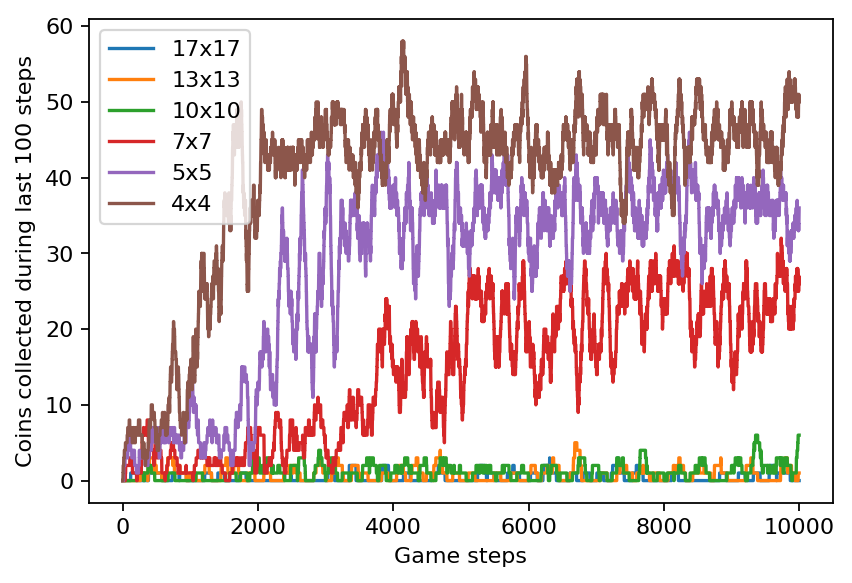
\includegraphics[width=\linewidth]{images/minigame-dense64-arch.png}
    \caption{Dense 64 (\ref{fig:dense-arch64})}
    \label{fig:network-dense64}
  \end{subfigure}
  \quad
  \begin{subfigure}[b]{0.48\linewidth}
    \centering
      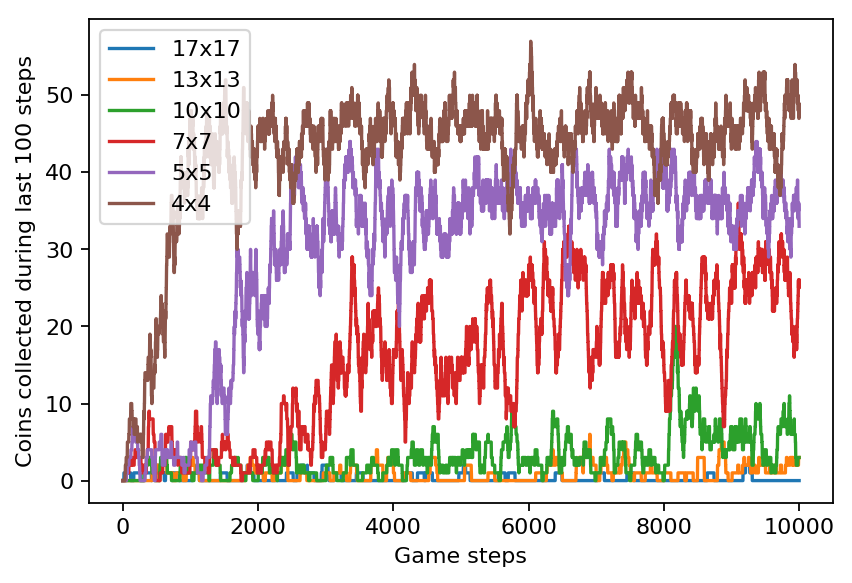
\includegraphics[width=\linewidth]{images/minigame-dense256-arch.png}
    \caption{Dense 256 (\ref{fig:dense-arch256})}
    \label{fig:network-dense256}
  \end{subfigure}
  \begin{subfigure}[b]{0.48\linewidth}
    \centering
    	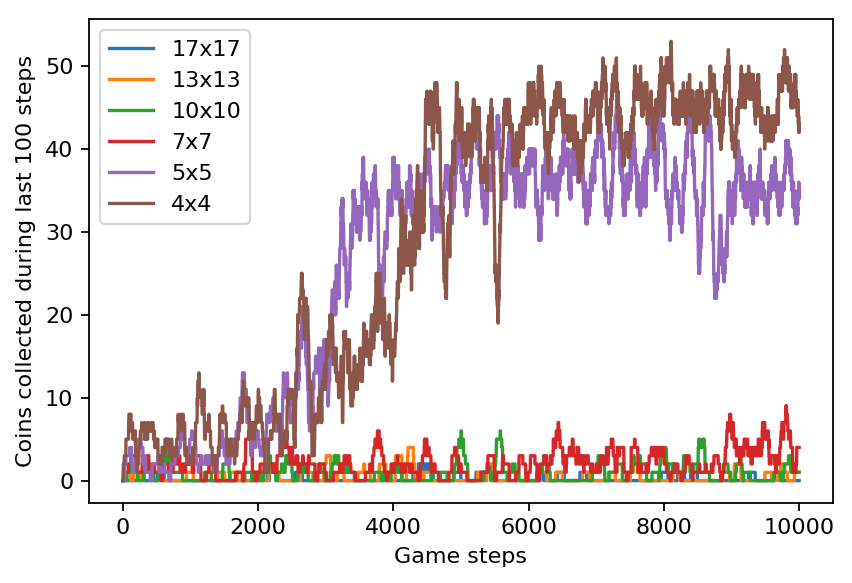
\includegraphics[width=\linewidth]{images/minigame-conv8-4-3-arch.png}
    \caption{Conv from Rainbow paper\cite{Hessel2018RainbowCI} (\ref{fig:conv-original})}
    \label{fig:network-conv843}
  \end{subfigure}
  \quad
  \begin{subfigure}[b]{0.48\linewidth}
    \centering
      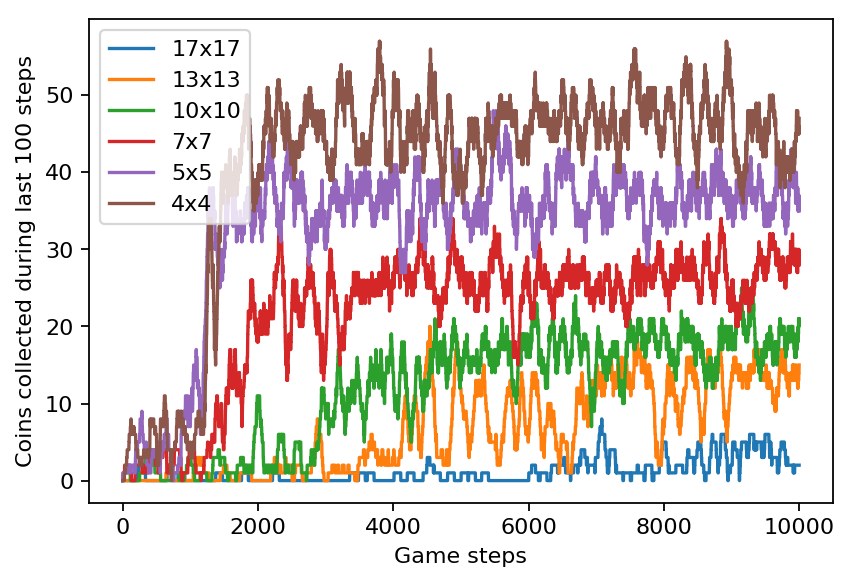
\includegraphics[width=\linewidth]{images/minigame-conv1-4-3-arch.png}
    \caption{Conv modified (\ref{fig:conv-modified})}
    \label{fig:network-conv143}
  \end{subfigure}
  \caption{Agents with different network architectures playing the minigame introduced in \ref{ch:minigame} for arena sizes from $4\times4$ to $17\times17$. There are three coins that can be collected per episode. The graphs show coins collected during the last 100 steps, continuing over episodes. For a big arena this number is naturally lower because of the large distances between coins, but it can be seen when and if the agent is plateauing.}
  \label{fig:networks}
\end{figure}



%!TEX root = ../bomberchamp.tex


\begin{figure}
  \centering
  \begin{subfigure}[b]{0.48\linewidth}
    \centering
	\begin{tabular}{l l l}
		\multicolumn{3}{c}{Shared network} \\
		\midrule
		Dense & 64 units & relu \\
		Dense & 64 units & relu \\
		\toprule
		\multicolumn{3}{c}{Advantage / value stream} \\
		\midrule
		NoisyDense & 64 units & relu \\
		\toprule
	\end{tabular}
    \caption{Dense 64}
    \label{fig:dense-arch64}
  \end{subfigure}
  \begin{subfigure}[b]{0.48\linewidth}
    \centering
	\begin{tabular}{l l l}
		\multicolumn{3}{c}{Shared network} \\
		\midrule
		Dense & 256 units & relu \\
		Dense & 256 units & relu \\
		\toprule
		\multicolumn{3}{c}{Advantage / value stream} \\
		\midrule
		NoisyDense & 256 units & relu \\
		\toprule
	\end{tabular}
    \caption{Dense 256}
    \label{fig:dense-arch256}
  \end{subfigure}
  \caption{Simple fully connected (dense) network. The last value and advantage stream layer is omitted.}
  \label{fig:dense-arch}
\end{figure}

%!TEX root = ../bomberchamp.tex

\begin{figure}
  \centering
  \begin{subfigure}[b]{0.48\linewidth}
    \centering
	\begin{tabular}{l l l l l}
		\multicolumn{5}{c}{Shared network} \\
		\midrule
		& $n_c$ & $f$ & $s$ & \\
		\midrule
		Conv2D & 32 & 8 & 4 & relu \\
		Conv2D & 64 & 4 & 2 & relu \\
		Conv2D & 64 & 3 & 1 & relu \\
		\toprule
		\multicolumn{5}{c}{Advantage / value stream} \\
		\midrule
		NoisyDense & \multicolumn{3}{l}{512 units} & relu \\
		\toprule
	\end{tabular}
    \caption{Conv from Rainbow paper\cite{Hessel2018RainbowCI}}
    \label{fig:conv-original}
  \end{subfigure}
  \begin{subfigure}[b]{0.48\linewidth}
    \centering
	\begin{tabular}{l l l l l}
		\multicolumn{5}{c}{Shared network} \\
		\midrule
		& $n_c$ & $f$ & $s$ & \\
		\midrule
		Conv2D & 32 & 1 & 1 & relu \\
		Conv2D & 64 & 4 & 2 & relu \\
		Conv2D & 64 & 3 & 2 & relu \\
		\toprule
		\multicolumn{5}{c}{Advantage / value stream} \\
		\midrule
		NoisyDense & \multicolumn{3}{l}{512 units} & relu \\
		\toprule
	\end{tabular}
    \caption{Modified convolutional NN}
    \label{fig:conv-modified}
  \end{subfigure}
  \caption{Convolutional network with number of channels $n_c$, filter size $f$ and stride $s$. The last value and advantage stream layer is omitted.}
  \label{fig:conv-arch}
\end{figure}

